% Options for packages loaded elsewhere
\PassOptionsToPackage{unicode}{hyperref}
\PassOptionsToPackage{hyphens}{url}
%
\documentclass[
  ignorenonframetext,
  aspectratio=169,
  fontset=ubuntu]{ctexbeamer}
\usepackage{pgfpages}
\setbeamertemplate{caption}[numbered]
\setbeamertemplate{caption label separator}{: }
\setbeamercolor{caption name}{fg=normal text.fg}
\beamertemplatenavigationsymbolsempty
\setbeameroption{show notes}
% Prevent slide breaks in the middle of a paragraph
\widowpenalties 1 10000
\raggedbottom
\setbeamertemplate{part page}{
  \centering
  \begin{beamercolorbox}[sep=16pt,center]{part title}
    \usebeamerfont{part title}\insertpart\par
  \end{beamercolorbox}
}
\setbeamertemplate{section page}{
  \centering
  \begin{beamercolorbox}[sep=12pt,center]{part title}
    \usebeamerfont{section title}\insertsection\par
  \end{beamercolorbox}
}
\setbeamertemplate{subsection page}{
  \centering
  \begin{beamercolorbox}[sep=8pt,center]{part title}
    \usebeamerfont{subsection title}\insertsubsection\par
  \end{beamercolorbox}
}
\AtBeginPart{
  \frame{\partpage}
}
\AtBeginSection{
  \ifbibliography
  \else
    \frame{\sectionpage}
  \fi
}
\AtBeginSubsection{
  \frame{\subsectionpage}
}
\usepackage{amsmath,amssymb}
\usepackage{iftex}
\ifPDFTeX
  \usepackage[T1]{fontenc}
  \usepackage[utf8]{inputenc}
  \usepackage{textcomp} % provide euro and other symbols
\else % if luatex or xetex
  \usepackage{unicode-math} % this also loads fontspec
  \defaultfontfeatures{Scale=MatchLowercase}
  \defaultfontfeatures[\rmfamily]{Ligatures=TeX,Scale=1}
\fi
\usepackage{lmodern}
\usecolortheme{thubeamer}
\usefonttheme{professionalfonts}
\useinnertheme{thubeamer}
\useoutertheme{thubeamer}
\ifPDFTeX\else
  % xetex/luatex font selection
\fi
% Use upquote if available, for straight quotes in verbatim environments
\IfFileExists{upquote.sty}{\usepackage{upquote}}{}
\IfFileExists{microtype.sty}{% use microtype if available
  \usepackage[]{microtype}
  \UseMicrotypeSet[protrusion]{basicmath} % disable protrusion for tt fonts
}{}
\makeatletter
\@ifundefined{KOMAClassName}{% if non-KOMA class
  \IfFileExists{parskip.sty}{%
    \usepackage{parskip}
  }{% else
    \setlength{\parindent}{0pt}
    \setlength{\parskip}{6pt plus 2pt minus 1pt}}
}{% if KOMA class
  \KOMAoptions{parskip=half}}
\makeatother
\usepackage{xcolor}
\newif\ifbibliography
\usepackage{longtable,booktabs,array}
\usepackage{calc} % for calculating minipage widths
\usepackage{caption}
% Make caption package work with longtable
\makeatletter
\def\fnum@table{\tablename~\thetable}
\makeatother
\usepackage{graphicx}
\makeatletter
\newsavebox\pandoc@box
\newcommand*\pandocbounded[1]{% scales image to fit in text height/width
  \sbox\pandoc@box{#1}%
  \Gscale@div\@tempa{\textheight}{\dimexpr\ht\pandoc@box+\dp\pandoc@box\relax}%
  \Gscale@div\@tempb{\linewidth}{\wd\pandoc@box}%
  \ifdim\@tempb\p@<\@tempa\p@\let\@tempa\@tempb\fi% select the smaller of both
  \ifdim\@tempa\p@<\p@\scalebox{\@tempa}{\usebox\pandoc@box}%
  \else\usebox{\pandoc@box}%
  \fi%
}
% Set default figure placement to htbp
\def\fps@figure{htbp}
\makeatother
\ifLuaTeX
  \usepackage{luacolor}
  \usepackage[soul]{lua-ul}
\else
  \usepackage{soul}
  \makeatletter
  \let\HL\hl
  \renewcommand\hl{% fix for beamer highlighting
    \let\set@color\beamerorig@set@color
    \let\reset@color\beamerorig@reset@color
    \HL}
  \makeatother
\fi
\setlength{\emergencystretch}{3em} % prevent overfull lines
\providecommand{\tightlist}{%
  \setlength{\itemsep}{0pt}\setlength{\parskip}{0pt}}
\setcounter{secnumdepth}{-\maxdimen} % remove section numbering
\hypersetup{colorlinks, allcolors=., urlcolor=blue,}
\usepackage{xeCJKfntef}
\providecommand{\st}[1]{\CJKsout{#1}}
\renewcommand{\st}[1]{\sout{#1}}
\usepackage{fvextra}
\usepackage[outputdir=tmp]{minted}
\usepackage{tcolorbox}
\usepackage{etoolbox}
\setminted{fontsize=\footnotesize,xleftmargin=0.7em,linenos,breaklines}
\renewcommand{\familydefault}{\sfdefault}
\addtobeamertemplate{note page}{}{\thispdfpagelabel{notes:\insertframenumber}}
\setCJKmonofont{Noto Sans Mono CJK SC}
\usepackage{bookmark}
\IfFileExists{xurl.sty}{\usepackage{xurl}}{} % add URL line breaks if available
\urlstyle{same}
\hypersetup{
  pdftitle={Test Slides},
  pdfauthor={陈晟祺},
  hidelinks,
  pdfcreator={LaTeX via pandoc}}

\title{Test Slides}
\subtitle{Using Pandoc to Write Beamer}
\author{陈晟祺}
\date{2024年8月27日}
\institute{清华大学 计算机科学与技术系}

\begin{document}
\frame{\titlepage}

\section{Introduction}\label{introduction}

\begin{frame}[fragile]{Introduction}
内含 Stata
基础功能、变量定义及内置命令、Dofiles,数据管理以及图表制作的相关技巧。本篇不涉及具体的数据回归与分析,更多的是一些规范工作流的命令。或许有一些指导意义,但更多的是健忘人士手册。
\end{frame}

\begin{frame}[fragile]{Let's get started!}
\phantomsection\label{lets-get-started}
\begin{block}{设置工作目录}
\phantomsection\label{ux8bbeux7f6eux5de5ux4f5cux76eeux5f55}
我承认最开始的时候我也是打开命令窗口直接开始
\mintinline[]{text}{import excel},直到我开始自己处理更大的数据和文件,才意识到设置工作目录并好好命名项目下的文件有多重要。朋友们,不要再设置中文的工作目录了,你永远不知道因为中文工作目录名称导致的报错会在哪一天以何种方式照进现实。

\begin{figure}
\centering
\pandocbounded{\includegraphics[keepaspectratio]{本人画了二十分钟的图无法保存!痛失可编辑图像一份。}}
\caption{/Users/thanksallthefish/Library/Mobile
Documents/iCloud\textsubscript{md}obsidian/Documents/Summer's
blog/source/asset/posts/Screenshot-2024-07-17-at-21.16.17@2x.png}
\end{figure}
\end{block}

\begin{block}{安装外部命令}
\phantomsection\label{ux5b89ux88c5ux5916ux90e8ux547dux4ee4}
当然这一步在遇到时再安装也是可以的,我真的只是为了让这篇文章看起来更像一个正确的实验设计才把他放在这里。

\begin{minted}[autogobble]{stata}
ssc install winsor2
\end{minted}
\end{block}
\end{frame}

\begin{frame}[fragile]{数据预处理}
\phantomsection\label{ux6570ux636eux9884ux5904ux7406}
\begin{block}{数据导入}
\phantomsection\label{ux6570ux636eux5bfcux5165}
\begin{minted}[autogobble]{stata}
import excel "data.xls", sheet("Sheet1") firstrow clear
\end{minted}

\begin{itemize}
\tightlist
\item
  \mintinline[]{text}{data.xls} 当前目录下原始 excel 文件
\item
  \mintinline[]{text}{sheet("Sheet1")}使用 Sheet1 页的数据
\item
  \mintinline[]{text}{firstrow} 以第一行作为变量名
\end{itemize}
\end{block}

\begin{block}{数据转换}
\phantomsection\label{ux6570ux636eux8f6cux6362}
\mintinline[]{text}{reshape}
命令绝对是我的噩梦。但事实是熟练之后在很多时候确实会 come in
handy。可惜的是我在一段时间没有用之后又不会了,这边建议日常 refer to
\mintinline[]{text}{help reshape} \st{for less brain damage}
\end{block}

\begin{block}{合并数据}
\phantomsection\label{ux5408ux5e76ux6570ux636e}
我一般用来把控制变量合并到核心变量的数据文件里去。\st{其实用 excel
也是可以的啊?}

\begin{minted}[autogobble]{stata}
merge 1:1 stkcd year using ControlVarsDetail, keep(3)
\end{minted}
\end{block}
\end{frame}

\begin{frame}[fragile]{说明}
\phantomsection\label{ux8bf4ux660e}
\begin{itemize}
\tightlist
\item
  \mintinline[]{text}{1:1} 1对1关联,\mintinline[]{text}{1:m}
  1对多关联,\mintinline[]{text}{m:1} 多对1关联
\item
  \mintinline[]{text}{id year}:根据 id 和 year
  这两个变量确定唯一值进行关联
\item
  \mintinline[]{text}{using}:使用要关联的数据集
\item
  \mintinline[]{text}{keep}:保留的意思,两份数据怎么进行关联,1:只保留主表没有关联上的数据,2:只保留副表没有关联上的数据,3:只保留主表和副表关联上的数据
\item
  例如 \mintinline[]{text}{keep(1 3)}
  表示保留主表没有关联上的数据和主表和副表关联上的数据
\item
  如遇到报错说主表或者关联表不是唯一值,则需要进行去除重复操作,\mintinline[]{text}{duplicates drop id year, force}
\end{itemize}
\end{frame}

\begin{frame}[fragile]{数据预处理}
\phantomsection\label{ux6570ux636eux9884ux5904ux7406-1}
\begin{block}{数据缩尾}
\phantomsection\label{ux6570ux636eux7f29ux5c3e}
对异常数据进行截尾,一般保留 1-99 百分位的数据

\begin{minted}[autogobble]{text}
winsor2 Y,cuts(1 99) trim replace
\end{minted}

该操作不可撤销(比如说我要是截尾了一次发现 1-99 不合适,想重新保留 5-95
百分位的数据该怎么办呢?呃,\st{我一般都是把 excel
里的原始数据再复制过来一遍})
\end{block}
\end{frame}

\begin{frame}[fragile]{标准化}
\phantomsection\label{ux6807ux51c6ux5316}
一个比较容易混淆的概念是标准化: - 缩放到 \([0, 1]\):

\[
   X_{\text{norm}} = \frac{X - \min(X)}{\max(X) - \min(X)}
\]

\begin{itemize}
\tightlist
\item
  缩放到 \([-1, 1]\) 范围 \[
   X_{\text{scaled}} = 2 \times \frac{X - \min(X)}{\max(X) - \min(X)} - 1
  \]
\end{itemize}
\end{frame}

\begin{frame}[fragile]{标准化}
\phantomsection\label{ux6807ux51c6ux5316-1}
假设你有一个变量 \mintinline[]{text}{X},Stata 具体步骤如下:

\begin{enumerate}
\item
  \textbf{计算最小值和最大值}:

  \begin{minted}[autogobble]{stata}
  summarize X
  \end{minted}
\item
  \textbf{标准化到{[}0, 1{]}范围}:

  \begin{minted}[autogobble]{stata}
  generate X_norm = (X - r(min)) / (r(max) - r(min))
  \end{minted}
\item
  \textbf{缩放到{[}-1, 1{]}范围}:

  \begin{minted}[autogobble]{stata}
  generate X_scaled = 2 * (X - r(min)) / (r(max) - r(min)) - 1
  \end{minted}
\end{enumerate}

\begin{block}{删除缺失值}
\phantomsection\label{ux5220ux9664ux7f3aux5931ux503c}
最后一步是删除缺失值,保存数据,比较简单代码就不放了。
\end{block}
\end{frame}

\section{Some tips that may be
useful}\label{some-tips-that-may-be-useful}

\begin{frame}[fragile]{历史记录}
\phantomsection\label{ux5386ux53f2ux8bb0ux5f55}
与 MATLAB 和其他终端不同,Stata 使用 \mintinline[]{text}{PageUp} 和
\mintinline[]{text}{PageDown} 键来浏览历史命令记录。学会这个之后 Summer
再也不用在历史窗口复制粘贴代码,\st{人类文明的一大步。}

在 Macbook
笔记本上可以通过以下组合快捷键操作。呃,为什么就不能设置个上下方向键呢。

\begin{minted}[autogobble]{text}
Windows:PgUp == Mac: fn/option(alt) + 上箭头
Windows:PgDn == Mac: fn/option(alt) + 下箭头

Windows:Home == Mac: fn + 左箭头
Windows:End == Mac: fn + 右箭头
\end{minted}
\end{frame}

\begin{frame}[fragile]{Niceness(内存优先级)}
\phantomsection\label{nicenessux5185ux5b58ux4f18ux5148ux7ea7}
\begin{minted}[autogobble]{stata}
set niceness 5 // default setting
\end{minted}

\mintinline[]{text}{niceness} 控制了 Stata
占用内存的程度,特别适用于大型计算任务(如 bootstrapping 或 multiple
imputations)。

\begin{figure}
\centering
\pandocbounded{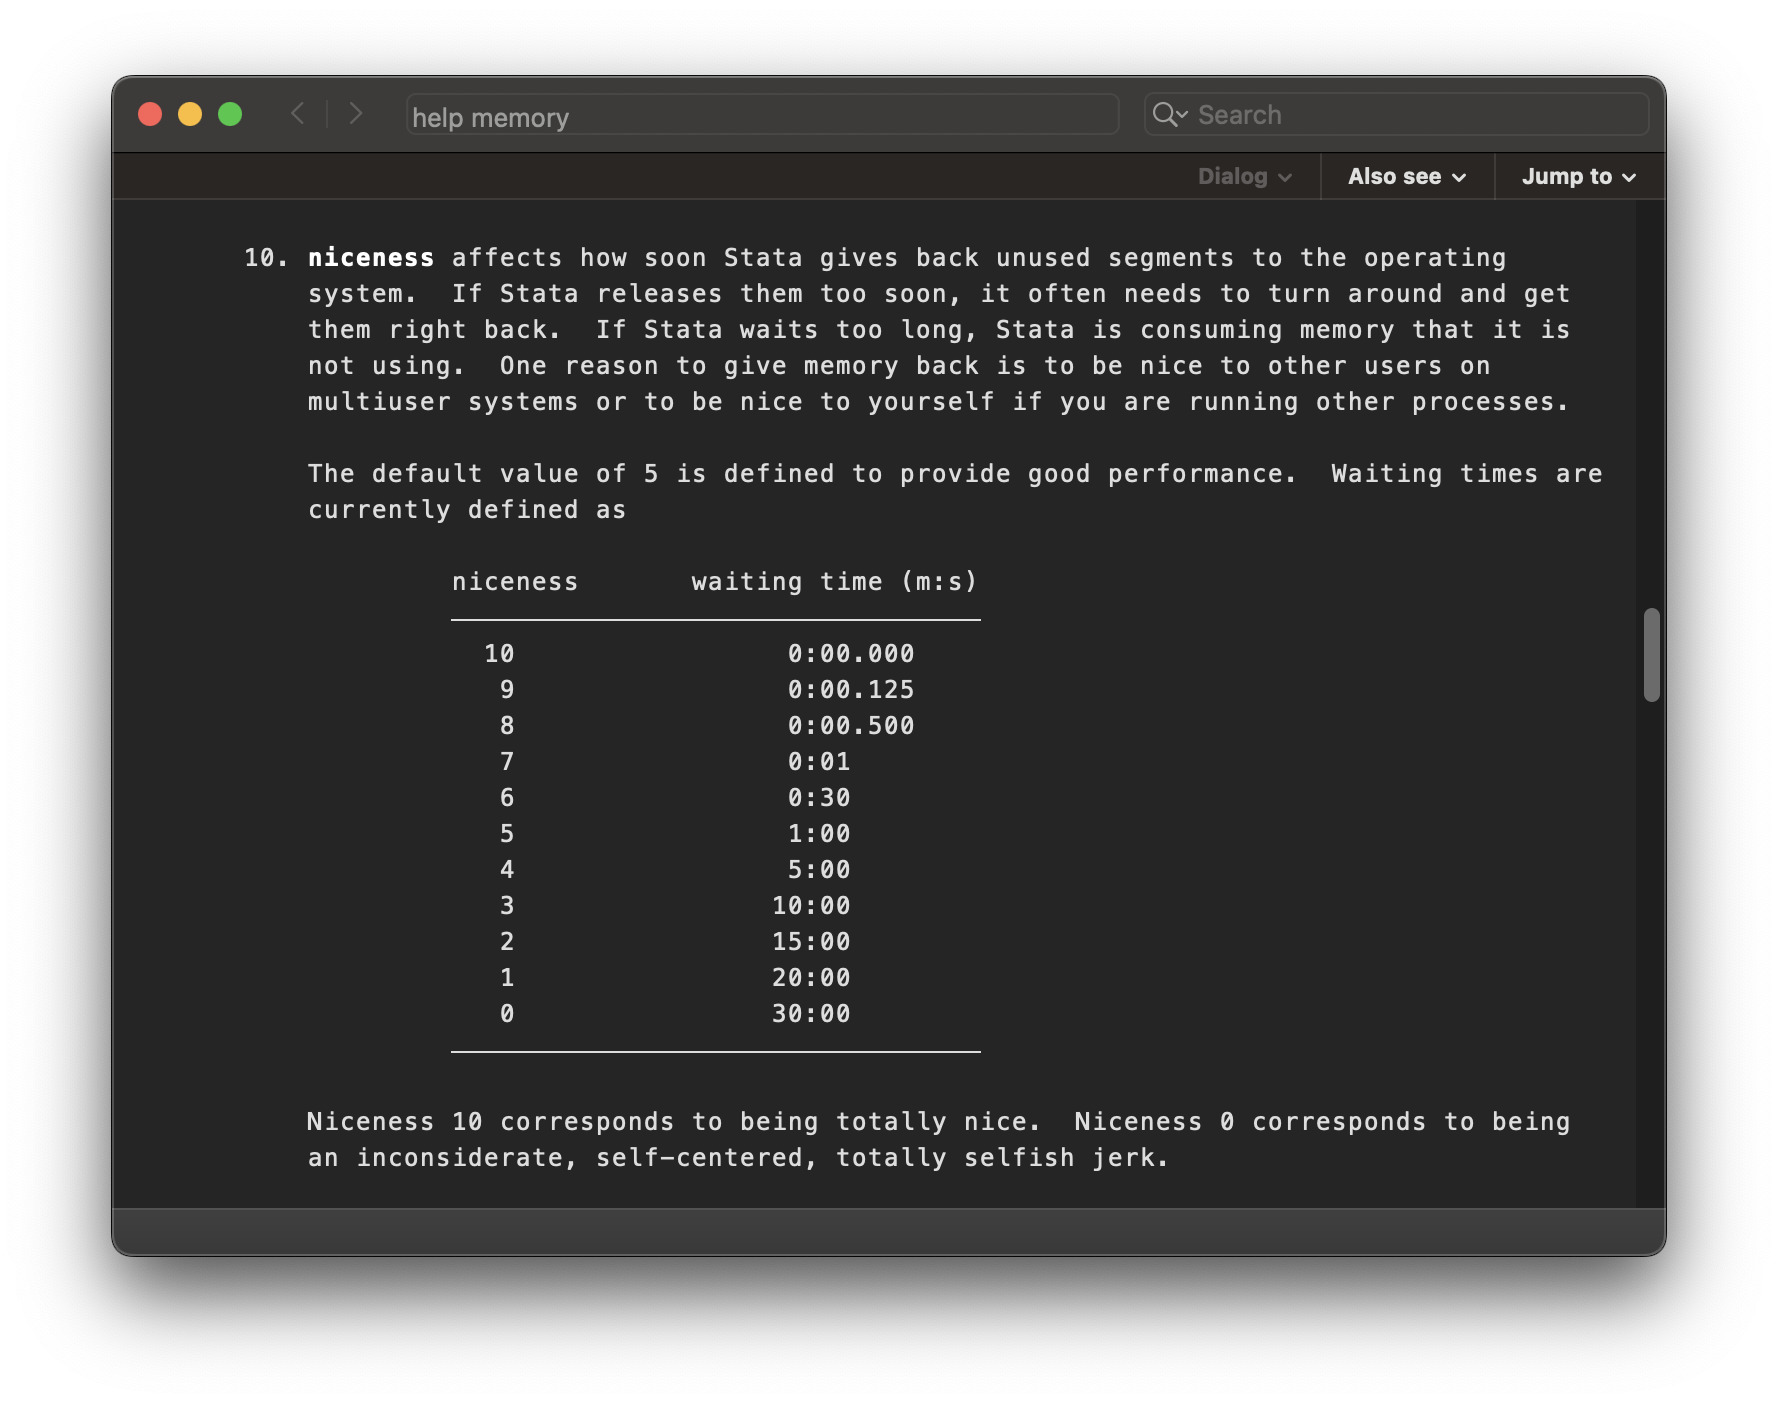
\includegraphics[keepaspectratio]{Screenshot-2024-07-17-at-19.53.04@2x.png}}
\caption{alt text}
\end{figure}
\end{frame}

\begin{frame}[fragile]{为图片命名}
\phantomsection\label{ux4e3aux56feux7247ux547dux540d}
为了避免新生成的图片覆盖旧图片,建议为每张图表设置名称,并使用
\mintinline[]{text}{autotabgraphs}
命令在单个窗口的多个标签页中打开图片:

\begin{minted}[autogobble]{stata}
set autotabgraphs on
set autotabgraphs on, perm  // for permanent changes
\end{minted}

尝试以下示例:

\begin{minted}[autogobble]{stata}
sysuse auto, clear
set autotabgraphs on
scatter price    mpg, name(graph1, replace)
scatter price length, name(graph2, replace)
set autotabgraphs off
scatter price    mpg, name(graph1, replace)
scatter price length, name(graph2, replace)
\end{minted}

启用 \mintinline[]{text}{autotabgraphs} 后,所有图表将以选项卡形式显示:

\pandocbounded{\includegraphics[keepaspectratio]{/Users/thanksallthefish/Library/Mobile Documents/iCloud~md~obsidian/Documents/Summer's blog/source/asset/posts/Screenshot-2024-07-17-at-19.54.17@2x.png}}
\end{frame}

\begin{frame}[fragile]{未记录的命令}
\phantomsection\label{ux672aux8bb0ux5f55ux7684ux547dux4ee4}
Stata
中有许多未记录的命令,其中一些非常有用。使用以下命令查看未记录命令(在这里轻轻推荐一下
\mintinline[]{text}{margins} 命令):

\begin{minted}[autogobble]{stata}
help undocumented
\end{minted}
\end{frame}

\begin{frame}[fragile]{为变量设置多语言}
\phantomsection\label{ux4e3aux53d8ux91cfux8bbeux7f6eux591aux8bedux8a00}
\st{成年人的崩溃往往就在一瞬间,比如说小朋友给你发来了一份全是以中文命名的变量的
dofile。看着头大不说,运行起来还会一堆报错。}其实在 Stata
里可以为变量和值不同语言的标签,而无需手动编辑数据集:

\begin{minted}[autogobble]{stata}
help label language
\end{minted}

我一般先把现有变量集命名为中文:

\begin{minted}[autogobble]{stata}
label language zh, rename

\end{minted}

再新建一个英文标签集慢慢改:

\begin{minted}[autogobble]{stata}
 label language en, new copy
\end{minted}

答应我,对于大型项目,一定要好好写变量标签。
\end{frame}

\begin{frame}[fragile]{设置小数点格式}
\phantomsection\label{ux8bbeux7f6eux5c0fux6570ux70b9ux683cux5f0f}
缘起于一位同学问我如何用 \mintinline[]{text}{set dp}
来控制输出结果的小数位数:

\begin{figure}
\centering
\pandocbounded{\includegraphics[keepaspectratio]{/Users/thanksallthefish/Library/Mobile Documents/iCloud~md~obsidian/Documents/Summer's blog/source/asset/posts/Pasted image 20240717171948.png}}
\caption{width:300px}
\end{figure}

然而这种使用方式是错误的,\mintinline[]{text}{set dp}
并没有控制输出结果小数位数的功能(要实现这个效果需要
\mintinline[]{text}{format}
命令),类似于上一条多语言功能,\mintinline[]{text}{set dp}
主要用于设置小数点和逗号的显示格式,例如在某些地区
\mintinline[]{text}{123,456.78} 会写作
\mintinline[]{text}{123.456,78}。正确的语法应该是:

\begin{minted}[autogobble]{stata}
set dp comma //设置小数点为逗号
\end{minted}
\end{frame}

\begin{frame}[fragile]{更新 ado 文件}
\phantomsection\label{ux66f4ux65b0-ado-ux6587ux4ef6}
使用以下命令可更新从 SSC 或其他方式安装和的自定义 ado 程序:

\begin{minted}[autogobble]{stata}
ado update
\end{minted}

我通常每个月都会运行一下,检查是否有纠正错误、添加功能的更新,以及重复安装的程序副本。

\pandocbounded{\includegraphics[keepaspectratio]{/Users/thanksallthefish/Library/Mobile Documents/iCloud~md~obsidian/Documents/Summer's blog/source/asset/posts/Screenshot-2024-07-17-at-17.37.16@2x.png}}
\end{frame}

\begin{frame}[fragile]{查找 Stata 数据集}
\phantomsection\label{ux67e5ux627e-stata-ux6570ux636eux96c6}
输入:

\begin{minted}[autogobble]{stata}
sysuse dir
\end{minted}

可查看 Stata 附带的所有数据集的列表。

\pandocbounded{\includegraphics[keepaspectratio]{/Users/thanksallthefish/Library/Mobile Documents/iCloud~md~obsidian/Documents/Summer's blog/source/asset/posts/Screenshot-2024-07-17-at-17.36.18@2x.png}}
\end{frame}

\begin{frame}[fragile]{timer: 查看命令运行所需时间}
\phantomsection\label{timer-ux67e5ux770bux547dux4ee4ux8fd0ux884cux6240ux9700ux65f6ux95f4}
我们可以使用内置的 \mintinline[]{text}{timer}
选项来测量一个或多个命令的执行时间:

\begin{minted}[autogobble]{stata}
webuse highschool, clear  
  
timer clear  
timer on 1  
svy: regress weight height  
timer off 1  
  
  
timer on 2  
svy: regress weight height sex  
timer off 2  
  
timer list
\end{minted}

可在一个计时器中运行多个命令。通过 \mintinline[]{text}{timer list}
输出可以获取每个计时器的执行时间。使用 \mintinline[]{text}{rmsg}
选项永久开启或关闭计时器选项。

\begin{minted}[autogobble]{stata}
. svy: regress weight height sex
(running regress on estimation sample)

Survey: Linear regression

Number of strata =  50                             Number of obs   =     4,071
Number of PSUs   = 100                             Population size = 8,000,000
                                                   Design df       =        50
                                                   F(2, 49)        =    315.01
                                                   Prob > F        =    0.0000
                                                   R-squared       =    0.2857

------------------------------------------------------------------------------
             |             Linearized
      weight | Coefficient  std. err.      t    P>|t|     [95% conf. interval]
-------------+----------------------------------------------------------------
      height |   .6071783    .041169    14.75   0.000      .524488    .6898686
         sex |  -7.965579   1.952784    -4.08   0.000    -11.88786   -4.043297
       _cons |  -90.30328   19.82128    -4.56   0.000    -130.1155   -50.49107
------------------------------------------------------------------------------

. timer off 2

. timer list
   1:     34.51 /        1 =      34.5080
   2:     13.98 /        1 =      13.9840

\end{minted}
\end{frame}

\section{优雅,不择手段的优雅!}\label{ux4f18ux96c5ux4e0dux62e9ux624bux6bb5ux7684ux4f18ux96c5}

\begin{frame}[fragile]{定义全局变量}
\phantomsection\label{ux5b9aux4e49ux5168ux5c40ux53d8ux91cf}
{答应我,花两分钟时间定义一下至少自变量和因变量。}

\begin{minted}[autogobble]{text}
*定义被解释变量,使用这个变量用$y表示
global y1 "Y1"
*定义解释变量,使用这个变量用$x表示
global x "X1"
*定义控制变量,使用这个变量用$control表示
global control "C1 C2 C3 C5 C6 C7"
*定义调节变量
global w "W"
*定义中介变量
global m "M"
*定义做稳健性检验的被解释变量
global y1 "Y2"
*定义做稳健性检验的解释变量
global x1 "X1"
*加入更多的控制变量
global otherControl "C8 C9 C10 C11"
*定义工具变量
global iv "IV"
\end{minted}

这样,在后续的代码中就不用再一个一个地敲变量名了。比如固定效应模型:

\begin{minted}[autogobble]{stata}
reghdfe $y $x $control, absorb(id year) vce(cluster id)

\end{minted}
\end{frame}

\begin{frame}[fragile]{重命名变量组}
\phantomsection\label{ux91cdux547dux540dux53d8ux91cfux7ec4}
Stata 的 \mintinline[]{text}{rename}
命令在最新版本中可以使用循环列表一次性重命名变量组:

\begin{minted}[autogobble]{stata}
  
// add an underscore to all variables  
sysuse auto, clear  
ren * *_  
  
// add an underscore to variables end with e  
sysuse auto, clear  
ren *e *e_
\end{minted}

参阅~\mintinline[]{text}{help rename}~了解更多自定义选项。
\end{frame}

\begin{frame}[fragile]{分段代码}
\phantomsection\label{ux5206ux6bb5ux4ee3ux7801}
使用大括号来折叠 \mintinline[]{text}{dofile} 中的代码块:

\begin{minted}[autogobble]{text}
{  
code block  
}
\end{minted}

对于那些只需偶尔检查或调试的代码段非常有用。

\pandocbounded{\includegraphics[keepaspectratio]{/Users/thanksallthefish/Library/Mobile Documents/iCloud~md~obsidian/Documents/Summer's blog/source/asset/posts/Screenshot-2024-07-17-at-21.20.01@2x.png}}
\end{frame}

\begin{frame}[fragile]{quietly}
\phantomsection\label{quietly}
接上,还可以使用带有大括号的 \mintinline[]{text}{quietly}
来抑制代码块的输出:

\begin{minted}[autogobble]{stata}
qui {
    <代码块>
}
\end{minted}
\end{frame}

\begin{frame}[fragile]{变量查找}
\phantomsection\label{ux53d8ux91cfux67e5ux627e}
如果数据集包含数百个变量,以下是几种有效的查找方法:

\begin{enumerate}
[(a)]
\tightlist
\item
  使用 \mintinline[]{text}{lookfor} 在变量名称和标签中搜索关键词:
\end{enumerate}

\begin{minted}[autogobble]{stata}
lookfor gender
\end{minted}

\begin{enumerate}
[(a)]
\setcounter{enumi}{1}
\tightlist
\item
  使用 \mintinline[]{text}{ds} 按变量类型进行搜索:
\end{enumerate}

\begin{minted}[autogobble]{stata}
ds, has(type numeric)
\end{minted}

这将列出所有数值类型的变量。也可以使用 \mintinline[]{text}{not}
选项排除特定类型的变量:

\begin{minted}[autogobble]{stata}
ds, not(type string)
\end{minted}

这条命令将给出除了字符串类型的变量外的所有变量。 \mintinline[]{text}{ds}
命令还可根据模式搜索和筛选变量,更多请参阅
\mintinline[]{text}{help ds}。
\end{frame}

\begin{frame}[fragile]{读取目录中的所有文件}
\phantomsection\label{ux8bfbux53d6ux76eeux5f55ux4e2dux7684ux6240ux6709ux6587ux4ef6}
在需要处理某个目录中大量不规则命名文件时,可以通过以下步骤快速找到目录中的所有文件:

\begin{minted}[autogobble]{stata}
local x: dir . files "*"
\end{minted}

或者,搜索特定类型的文件,比如只查找 \mintinline[]{text}{.csv} 文件:

\begin{minted}[autogobble]{stata}
local x: dir . files "*.csv"
\end{minted}

显示查找到的文件列表:

\begin{minted}[autogobble]{stata}
display "`x'"
\end{minted}

我在处理公司年报文件时会经常使用这个命令。
\end{frame}

\begin{frame}[fragile]{优化条件表达式}
\phantomsection\label{ux4f18ux5316ux6761ux4ef6ux8868ux8fbeux5f0f}
既然我们要不择手段的优雅了,那总归是要了解一些 condition
相关的命令。比如当需要基于多个条件生成变量时可以这样写:

\begin{minted}[autogobble]{stata}
gen y = 1 if inlist(x, 1, 2, 5) // 如果 `x` 的值在集合 {1, 2, 5} 中,那么 `gen y = 1`。
\end{minted}

当然,一个个列举条件(如
\mintinline[]{text}{x==1 | x==2 | x==5})也是可以的了,但这样会有两个问题:1、数据多或者条件多了之后,运算速度会大幅下降,2、不够优雅。

对于连续变量也可有:

\begin{minted}[autogobble]{stata}

// 对于连续变量 mpg,生成多个条件变量
sysuse auto
gen v1 = mpg > 20        // v1: mpg 大于 20 的情况下为 1,否则为 0
gen v2 = !inrange(mpg, 0, 20) // v2: mpg 不在 0 到 20 范围内为 1,否则为 0
gen v3 = cond(mpg > 20, 1, 0) // v3: mpg 大于 20 的情况下为 1,否则为 0
recode mpg (0/20 = 0) (21/. = 1), gen(v4) // v4: 将 mpg 从 0 到 20 的范围重新编码为 0,21 到最大值的范围编码为 1
gen v5 = irecode(mpg, 0, 20, .) // v5: 使用 irecode 将 mpg 重新编码为 0(小于 0)、2(大于 20)或缺失值(如果是缺失值)


\end{minted}

使用 \mintinline[]{text}{inrange} 函数来代替逻辑表达式:

\begin{minted}[autogobble]{stata}
gen v6 = inrange(mpg, 1, 10)
\end{minted}

这种方式比使用逻辑运算符 \mintinline[]{text}{&} 和比较运算符
\mintinline[]{text}{>=} 和 \mintinline[]{text}{<=}
编写条件表达式更加简洁和直观。

推荐查阅这几个命令的帮助文件去优化条件表达式的书写。Stata
的官方文档写得非常难读,有的时候也可以直接 Google。
\end{frame}

\begin{frame}[fragile]{inspect: 快速检查变量}
\phantomsection\label{inspect-ux5febux901fux68c0ux67e5ux53d8ux91cf}
如果想快速了解变量的完整性和分布情况,请使用
\mintinline[]{text}{inspect}。它类似于
\mintinline[]{text}{summarize},但会在结果窗口中展示直方图。

\begin{minted}[autogobble]{stata}
sysuse auto 
summ weight 
inspect weight
\end{minted}
\end{frame}

\begin{frame}[fragile]{Heatplot}
\phantomsection\label{heatplot}
在 Stata 中可视化 Mata 矩阵可以通过 Ben Jann 的
\mintinline[]{text}{heatplot}
命令来实现(\mintinline[]{text}{ssc install heatplot})。

\begin{minted}[autogobble]{stata}
mata A = runiform(10, 10)  
heatplot mata(A)           
\end{minted}

以上命令表示:创建一个 10x10 的随机矩阵,使用 heatplot 命令可视化矩阵
A。图中展示矩阵 \mintinline[]{text}{A}
中各个元素的数值,颜色越深表示数值越大,颜色越浅表示数值越小。

\pandocbounded{\includegraphics[keepaspectratio]{/Users/thanksallthefish/Library/Mobile Documents/iCloud~md~obsidian/Documents/Summer's blog/source/asset/posts/Screenshot-2024-07-17-at-20.09.15@2x.png}}

在做\textbf{方差-协方差矩阵}和\textbf{空间误差项}矩阵中用的比较多。
\end{frame}

\begin{frame}[fragile]{clear vs.~clear all}
\phantomsection\label{clear-vs.-clear-all}
在 Stata 中,\mintinline[]{text}{clear} 与
\mintinline[]{text}{clear all} 或 \mintinline[]{text}{clear *}
是不同的。大多数人使用 \mintinline[]{text}{clear}
来清除当前数据集和标签,而 \mintinline[]{text}{clear all}
则会彻底清除所有记录。在处理矩阵、mata、框架、程序等时,使用
\mintinline[]{text}{clear all} 以确保清除整个工作环境。
\end{frame}

\begin{frame}[fragile]{gtools}
\phantomsection\label{gtools}
\href{https://gtools.readthedocs.io/en/latest/}{gtools}
套件的操作速度极快,能够在非常短的时间内完成对大规模数据集的
\mintinline[]{text}{reshape} 和 \mintinline[]{text}{collapse} 操作。
\end{frame}

\begin{frame}[fragile]{利用正则表达式清洗数据}
\phantomsection\label{ux5229ux7528ux6b63ux5219ux8868ux8fbeux5f0fux6e05ux6d17ux6570ux636e}
\begin{minted}[autogobble]{stata}
* 检查post是否还有其他非数字字符
list post if regexm(post, "[^0-9]")
\end{minted}

又例如:

\begin{minted}[autogobble]{stata}
* 消除字符串变量中所有额外的空格/制表符
x2= trim(ustrregexra(x,"/(\r\n\t)+|\r+|\n+|\t+/", ""))
* 将 x2 的多个连续空格或制表符替换为单个空格
gen x3 = ustrregexra(x2,"[ \t]+|[ \t]+", " ")
\end{minted}

正则表达式真是伟大的发明!
\end{frame}

\section{数据分析}\label{ux6570ux636eux5206ux6790}

\begin{frame}[fragile]{数据分析}
整了半天终于可以开始数据分析了。但是我说了这篇文章不涉及具体的数据分析,故在此只列一下数据分析的大概框架,等我把目前的东西写完了再整理这部分相关的有用技巧\st{以及让结果显著的旁门左道}。

\begin{enumerate}
\tightlist
\item
  描述性统计
\item
  相关性分析
\item
  多重共线性检验
\item
  基准回归
\item
  稳健性检验

  \begin{enumerate}
  \tightlist
  \item
    替换被解释变量
  \item
    替换解释变量(不适用于 DID)
  \item
    加入更多的固定效应
  \item
    修改稳健标准误
  \item
    增减样本量
  \item
    加入更多的控制变量
  \item
    调整样本周期
  \item
    剔除特殊年份
  \item
    剔除特殊样本
  \item
    X 滞后一期
  \item
    用插值法处理缺失值后回归
  \item
    改变缩尾水平
  \end{enumerate}
\item
  适用于 DID 的稳健性检验

  \begin{enumerate}
  \tightlist
  \item
    安慰剂,虚构时间、虚构处理组
  \item
    PSM-DID
  \item
    平行趋势检验
  \item
    平行趋势敏感性分析
  \item
    排他性检验
  \item
    异质性处理效应(好几种,包括 SDID)
  \item
    单期-多期呼唤
  \item
    当期换成小数
  \item
    预期效益检验
  \item
    三重差分 DDD
  \end{enumerate}
\item
  内生性

  \begin{enumerate}
  \tightlist
  \item
    工具变量法(用好很难)
  \item
    PSM
  \item
    安慰剂检验
  \item
    Heckman 二阶段
  \item
    断点回归 RDD
  \item
    广义矩估计
  \item
    DID
  \item
    熵平衡法检验(Hainmueller J, 2012)
  \end{enumerate}
\item
  机制检验

  \begin{enumerate}
  \tightlist
  \item
    调节效应
  \item
    中介效应(目前争议很大!Refer to 江艇, 2022)
  \end{enumerate}
\item
  异质性分析 一定要写清楚为什么要这样分类啦!
\end{enumerate}
\end{frame}

\begin{frame}[fragile]{安慰剂检验}
\phantomsection\label{ux5b89ux6170ux5242ux68c0ux9a8c}
不知道各位有没有偶尔 Emo
的时候会想到,假如当年好好学习,或者当年勇敢一点,会不会今天的我们就不一样了呢?

那么此时我们就得到一个因果关系:

\[\text{不好好学习,怂} \xrightarrow{\text{导致}} \text{今天的我}\]
这时候让时光倒流 1000 次,给你 1000
次重新选择的机会,那么这个时候你选择了好好学习,选择了那个时候勇敢一点,而结果是在
1000 次中,有好多好多次都成为了理想的自己

\[\text{好好学习,勇敢一点} \xrightarrow{\text{成为}} \text{理想的我}\]

那么此时我们就可以反推:确实是不好好学习、怂导致了今天的自己。那么此时安慰剂经验就是通过的了。
但是生活中没有如果,往往是好好学习、再勇敢一点,进行了哪怕1000次,会发现有些东西就是命中注定,自己还是自己:
\[\text{好好学习,勇敢一点} \xrightarrow{\text{}} \text{我还是我}\]
那么这个时候安慰剂检验就没有通过。也就是说无论是否好好学习,无论是否勇敢,仍然都导致了今天的自己,可能任何
X 都可能导致这个 Y,这两者的因果关系并不成立。

安慰剂检验结果看两点: 1. 如果汇报系数,虚假系数在 0 附近 2.
真实系数离原虚假的结果很远,表示基准结果不是随机能得到的
\end{frame}

\begin{frame}[fragile]{替换变量}
\phantomsection\label{ux66ffux6362ux53d8ux91cf}
\begin{enumerate}
\tightlist
\item
  虚构解释变量

  \begin{enumerate}
  \tightlist
  \item
    条件性虚构(按照城市)
  \item
    直接随机分配,包括 DID
  \end{enumerate}
\item
  虚构被解释变量

  \begin{enumerate}
  \tightlist
  \item
    另外找一个新的 Y
  \item
    直接随机分配
  \end{enumerate}
\item
  虚构处理时间(DID)
\item
  虚构处理组(DID)
\end{enumerate}

3、4 单期和多期又不一样
\end{frame}

\begin{frame}[fragile]{增加固定效应或时间趋势项}
\phantomsection\label{ux589eux52a0ux56faux5b9aux6548ux5e94ux6216ux65f6ux95f4ux8d8bux52bfux9879}
基准:企业+年份固定效应

稳健性检验: -
考虑地区层面的因素,加入城市、城市X年份(张形.企业所得税间接优惠与纳税遵从度山.当代经济科学,2023,45(01):130-140.)
-
排除同期环境规制政策的影响:城市年份、行业X年份(喻旭兰,周颖.绿色信贷政策与高污染企
业绿色转型:基于减排和发展的视角山.数量经济技术经济研究.2023.40(7):179-200.)

由此衍生出一个非常相似的方法: -
城市X年份{趋势}固定效应(韩先锋,魏欣,肖远飞.科技金融政策赋能城市数字技术创新---基于``科技和金融结合试点〞的经验证据.金融理论与实践,2024,(5):34-45:2024-07-171.)

\begin{block}{时间固定效应 vs.~时间趋势固定效应}
\phantomsection\label{ux65f6ux95f4ux56faux5b9aux6548ux5e94-vs.-ux65f6ux95f4ux8d8bux52bfux56faux5b9aux6548ux5e94}
\begin{enumerate}
\tightlist
\item
  控制每年的特征(i. 不分大小) 生成虚拟变量:
\end{enumerate}

\begin{longtable}[]{@{}llll@{}}
\toprule\noalign{}
& \(Year2015\) & \(Year2016\) & \(Year2017\) \\
\midrule\noalign{}
\endhead
2015 & 1 & 0 & 0 \\
2016 & 0 & 1 & 0 \\
2017 & 0 & 0 & 1 \\
\bottomrule\noalign{}
\end{longtable}

加入到模型: \[
reg \quad y \quad x \quad cvs \quad Year2015 \quad Year2016 \quad Year2017
\]

常见的:

\$\$ \begin{align*}
reg \quad \dots \underline{i.year}  \\
xtreg \quad \dots \underline{i.year}  \\
reghdfe \quad \dots , \underline{a(year)}
\end{align*}

\$\$

\begin{enumerate}
\setcounter{enumi}{1}
\tightlist
\item
  考虑时间趋势变化(c.~分大小)
\end{enumerate}

把时间(如2015、2016)放到回归之中

Reg y x cvs year i.year\ldots. xtreg y x cvs year i.year \ldots. reg y x
cvs c.year i.year xtreg y x cvs c.year i.year
\end{block}

\begin{block}{小结}
\phantomsection\label{ux5c0fux7ed3}
\begin{enumerate}
\tightlist
\item
  加入地区单项固定 (城市固定、省份固定):i.城市 i.省份
\item
  加入与年份的联合固定(行业、地区×年份):\mintinline[]{text}{i.城市 #i.年份},\mintinline[]{text}{i.省份#i.年份}
\item
  加入时间趋势单项(三种方式)\mintinline[]{text}{c.趋势项}
\item
  加入企业、行业、地区的虚拟变量与时间超势的交互项\mintinline[]{text}{i.城市#c.年份  i省份#c.年份}
\end{enumerate}
\end{block}

\begin{block}{注}
\phantomsection\label{ux6ce8}
\begin{enumerate}
\tightlist
\item
  以上在期刊论文中不常用作稳健性,而是放在基准回归里丰富列数,但用在毕业论文里还是可以的。
\item
  对于``加入地区单项固定'',显著性、系数变化不大,没啥意义\st{(没意义=显著=能毕业=好方法)}
\item
  加入与年份的联合固定,年份单项固定就不需要了(个人观点)
\end{enumerate}

我就说不能在这一篇里写具体操作。。打住打住以后再写
\end{block}
\end{frame}

\section{论文写完了,画图!}\label{ux8bbaux6587ux5199ux5b8cux4e86ux753bux56fe}

\begin{frame}[fragile]{论文写完了,画图!}
挑几个我最喜欢的命令说说。
\end{frame}

\begin{frame}[fragile]{坐标轴自动缩放}
\phantomsection\label{ux5750ux6807ux8f74ux81eaux52a8ux7f29ux653e}
在定期更新图表(例如 COVID-19
时间序列信息)时,可以通过使用变量的最小值和最大值来自动调整轴的范围:

\begin{minted}[autogobble]{stata}
// 获取日期变量的摘要统计信息
summ date

// 设置 x1 为日期变量的最小值
local x1 = `r(min)'

// 设置 x2 为日期变量的最大值
local x2 = `r(max)'

// 自动调整 x 轴的标签范围
xlabel(`x1'(10)`x2')
\end{minted}

如果想要在轴的最大值上增加一些空间:

\begin{minted}[autogobble]{stata}
summ date  
  local x1 = `r(min)'  
  local x2 = `r(max)' + 30
xlabel(`x1'(10)`x2')
\end{minted}

就可以在右边添加一些你想要的标签啦。
\end{frame}

\begin{frame}[fragile]{设置图表刻度数}
\phantomsection\label{ux8bbeux7f6eux56feux8868ux523bux5ea6ux6570}
与其自定义坐标轴范围,也可以直接指定所需的刻度数,例如:

\begin{minted}[autogobble]{stata}

sysuse auto, clear
twoway (scatter price mpg), xlabel(#20) ylabel(#20)
\end{minted}

以上代码表示绘制散点图,并设置 x 轴和 y 轴的刻度数为 20。

\pandocbounded{\includegraphics[keepaspectratio]{/Users/thanksallthefish/Library/Mobile Documents/iCloud~md~obsidian/Documents/Summer's blog/source/asset/posts/Screenshot-2024-07-17-at-21.01.01@2x.png}}
\end{frame}

\begin{frame}[fragile]{指定图例顺序}
\phantomsection\label{ux6307ux5b9aux56feux4f8bux987aux5e8f}
例如按指定顺序显示图例中的第 5、第 3 和第 1 个元素:

\begin{minted}[autogobble]{stata}

legend(order(5 "var5" 3 "var3" 1 "var1"))
\end{minted}
\end{frame}

\begin{frame}[fragile]{在图片中添加文本框}
\phantomsection\label{ux5728ux56feux7247ux4e2dux6dfbux52a0ux6587ux672cux6846}
好像很少有人提到这一点,我也是在读帮助文档时偶然读到的,\st{没有用的技能增加了。}

\begin{minted}[autogobble]{stata}
twoway (scatter mpg weight), text(35 4200 "这是一些说明文字" "这是另外的说明文字", size(small) box just(left) margin(l+2 t+2 b+2) fcolor(gs14%80) lw(none))
\end{minted}

\pandocbounded{\includegraphics[keepaspectratio]{/Users/thanksallthefish/Library/Mobile Documents/iCloud~md~obsidian/Documents/Summer's blog/source/asset/posts/Screenshot-2024-07-17-at-21.40.51@2x.png}}
\end{frame}

\end{document}
